\section{Introduction}
\label{sec:introduction}

\begin{itemize}
	\item Past traffic analysis attempts focused only on TCP streams.
	\item Associated traffic such as DNS is an issue, because its distributed
		nature greatly increases path coverage, i.e., the number of ASes that
		are traversed by IP packets.
	\item As a result, past work might have underestimated the impact of
		network-level adversaries.
\end{itemize}

Questions:
\begin{itemize}
	\item What's the additional path coverage of DNS requests, i.e., how much
		easier does the job of a network-level adversary become?
	\item Can a global passive adversary correlate single DNS requests?  What's
		the false positive rate?
	\item How do we best mitigate these issues?  What can we recommend to exit
		relay operators?
	\item What's the probability of ending up with a guard/exit combination that
		makes us fall prey to relay-level adversaries?
	\item How many exit relays use EDNS?
	\item What resolvers are used by exit relays?
\end{itemize}

Possible contributions:
\begin{itemize}
	\item We show how DNS can help adversaries perform end-to-end correlation.
	\item We shed light on how Tor exit relays perform DNS resolution.
\end{itemize}

Available data:
\begin{itemize}
	\item DNS resolvers of exit relays over time (see \S~\ref{sec:dns-resolver-dataset}).
	\item DNS requests captured by DNS root (see \S~\ref{sec:dns-root-dataset}).
	\item Traceroutes from (near) exits to destinations (see \S~\ref{sec:traceroute-dataset}).
\end{itemize}

Things that could help us demonstrate an attack:
\begin{itemize}
	\item Traffic analysis done on an entry guard.  Can DNS requests be isolated
		reliably?
	\item Access to DNS root, .com, and .net.
	\item Ability to use DNS resolver's cache as an oracle.
	\item Ability to enumerate what resolver's an exit relay uses.
	\item Resolvers using EDNS.
	\item Users in country X are likely to resolve domains of country X.
\end{itemize}

\begin{figure}[t]
	\centering
	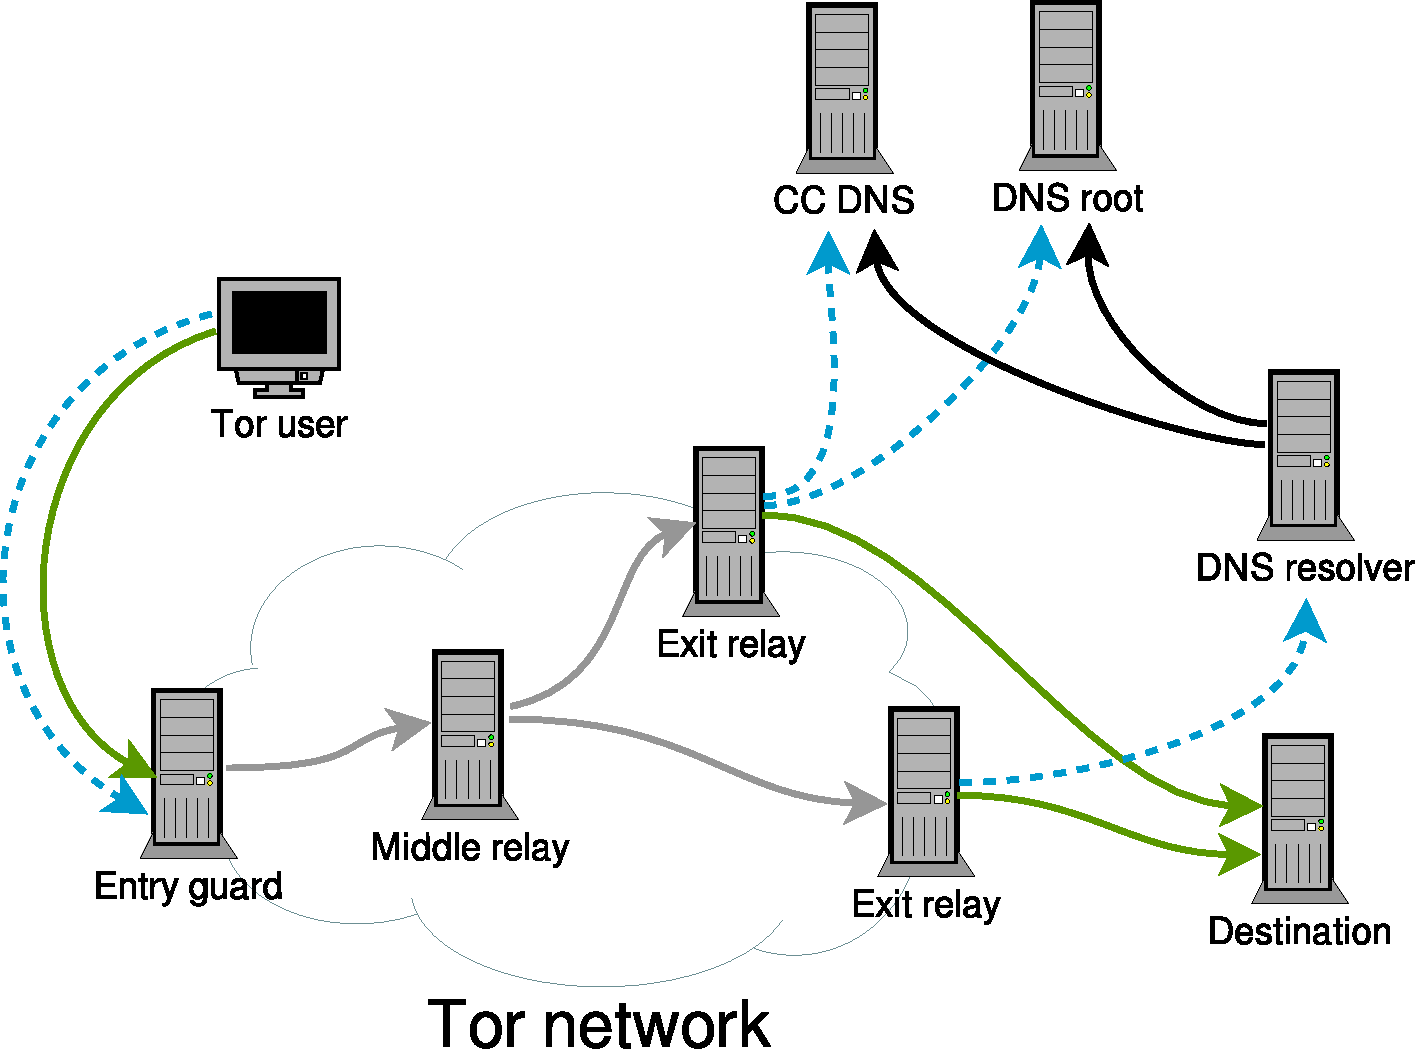
\includegraphics[width=0.45\textwidth]{figures/overview.pdf}
	\label{fig:overview}
	\caption{Traditional approaches to traffic analysis have focused on linking
	the TCP stream entering the network to the one exiting the network (green,
	solid lines).  We show that associated DNS traffic (blue, dotted lines) can
	also be linked, and is exposed to more parties than the TCP stream.}
\end{figure}
